\section{Experiments}
\subsection{Datasets}
To test my model I used two image datasets. I chose to use image data because they have a large number of features, even for simple images, and noise can be easily added artificially. In particular, I ran my experiments on the MNIST \cite{mnist} and EMNIST \cite{emnist} datasets (Figure \ref{fig:datasets}). MNIST is a classical dataset in image processing which consists of 60,000 handwritten digits displayed in 28x28 gray-scale images. EMNIST (extended MNIST) is a recent dataset which consists of images in the same format as MNIST, but includes letters A-Z as well as digits. For this work, I only considered the 124,800 images from the dataset which were of a letter. Letters in the dataset can be upper or lowercase, however, there is only 26 classes. That is, images of ``a" and ``A" are considered the same class.

\begin{figure}
	\centering
	\begin{subfigure}[b]{\textwidth}
		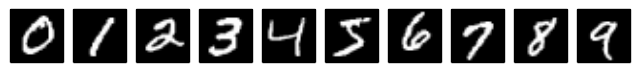
\includegraphics[width=\textwidth]{figs/mnist.png}
	\end{subfigure}
	\begin{subfigure}[b]{\textwidth}
		
\includegraphics[width=\textwidth]{figs/emnist.png}
	\end{subfigure}
	\caption{Sample images. MNIST (upper) consists of handwritten digits 0-9 and EMNIST (lower) consists of handwritten letters a-z and A-Z. Both consist of 28x28 centered gray-scale images.}
	\label{fig:datasets}
\end{figure}

\subsection{Implementation Details}
All my experiments and models were developed using Tensorflow\footnote{\texttt{https://www.tensorflow.org}} (my code is publicly available\footnote{\texttt{https://github.com/colinski/AutoencodedKMeans}}). For both datasets a batch size of 100 was used. Optimization was performed via the Adam optimizer \cite{adam} using the default parameters of the Tensorflow implementation\footnote{\texttt{https://www.tensorflow.org/api\_docs/python/tf/train/AdamOptimizer}}. The number of clusters used was determined to be 10 times the number of classes, so 100 for MNIST and 260 for EMNIST. The autoencoder used a tanh nonlinearity. The matrix of cluster centers was initialized as the pseudo-identity matrix, and the weights and biases of the autoencoder was initialized using the Xavier initialization method \cite{xavier}. Training took place on a GPU.

\subsection{Effect of Representation Dimension}
We first experiment by changing the size of the representation produced by the autoencoder. For a range of values (2 at the lowest, 400 at the highest), I trained autoencoded $k$-means to learn a representation of that size and simultaneously cluster the data in that smaller dimensional feature space. We hope that the autoenocder will select the most informative features, resulting in better clustering. The results of these experiments can be found in Figure \ref{fig:dims}

We see a significant decrease in performance on both datasets for small dimensional values (2 and 64) when compared to $k$-means. This isn't surprising since it seems unlikely that a 784 feature space could be reasonably represented in 2. However, once a reasonable dimension size is reached, we see an increase in performance  on both datasets. MNIST especially shows sizable gains over $k$-means for a dimension of size 256. Interestingly, as the dimension size increases past 256, we see a drop in performance on the MNIST data. This suggests that the autoencoder may be preserving unimportant features in its representation, leading to worse clustering performance.

From these experiments we see that EMNIST is significantly harder dataset to cluster. This isn't surprising given the increased complexity of the data. Autoencoded $k$-means is able to gain a small performance gain over $k$-means, however it scores consistently worse on the V-Measure metric, across all choices of dimension size. This is due to the fact that the completeness component of the V-Measure on the EMNIST data was consistently low. This means that points from the same class aren't being assigned to the same cluster. This may be due to the fact that EMNIST treats upper and lowercase letters as the same class. It seems likely that autoencoded $k$-means is learning to place ``a" in a different cluster than ``A", resulting in lower completeness.

\begin{figure}
	\centering
	\begin{minipage}[b]{0.45\textwidth}
		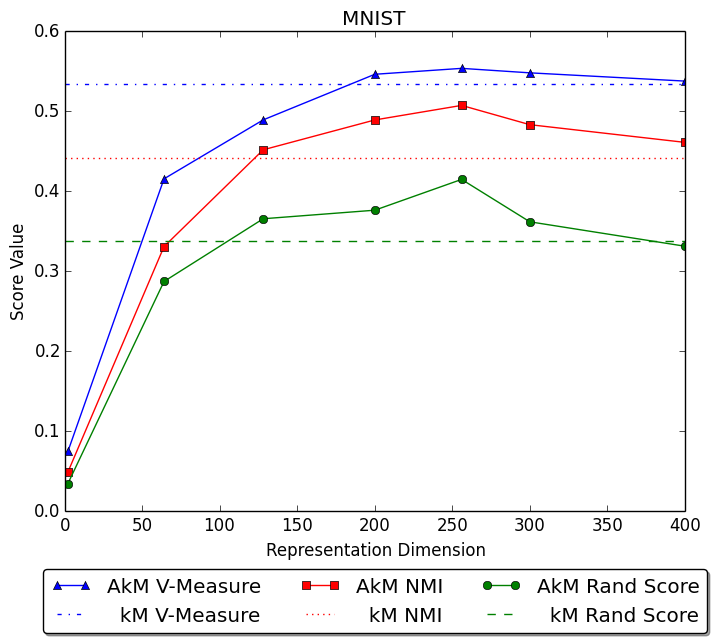
\includegraphics[width=\textwidth]{figs/mnist_graph.png}
	\end{minipage}
	\hfill
	\begin{minipage}[b]{0.45\textwidth}
		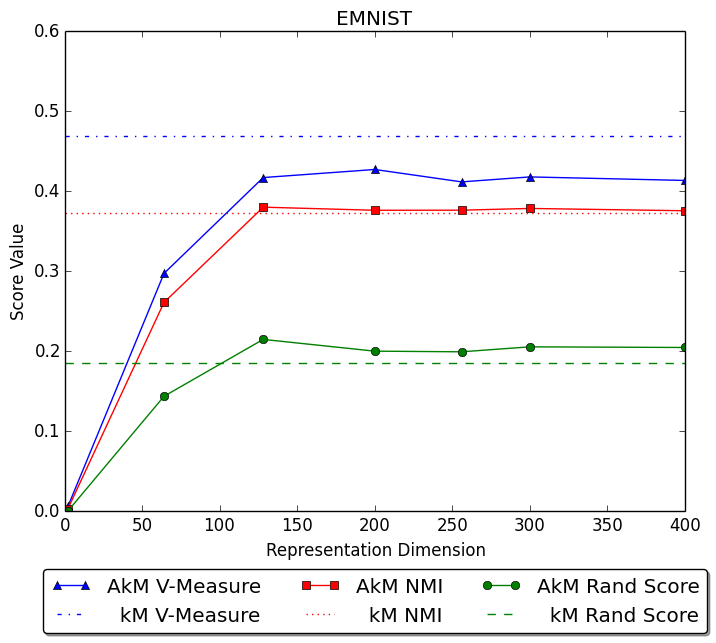
\includegraphics[width=\textwidth]{figs/emnist_graph.png}
	\end{minipage}
	\caption{Effect of representation dimension on performance. Solid lines show score values from the clusterings generated by autoencoded $k$-means (AkM). Horizontal dashed lines show score values of clusterings produced by gradient $k$-means (kM) without any autoencoder.}
	\label{fig:dims}
\end{figure}

\subsection{Effect of Noisy Data}
To evaluate the capacity  of my model to denoise data, I artificially added noise to the images. I applied a technique known as Gaussian whitening. For each pixel, a value was drawn from a zero mean Gaussian distribution with variance $\sigma^2$. This value was added to the pixel's value and then clipped so it falls in a valid range for the image (0-255). Increasing the variance results in nosier images. Figure \ref{fig:noisy} shows examples of such images. For values of $\sigma^2$ from 0 to 100, I generated a noisy dataset and trained autoencoded $k$-means to denoise this data. The best performing dimension size (256 for MNIST and 128 for EMNIST) from the previous experiments were used. Therefore autoencoded $k$-means is in fact simultaneously reducing the dimensionality of the data and denoising it. Figure \ref{fig:noise} shows that results of these experiments.

We first discuss the performance of $k$-means on noisy data. From my experiments we see that it performs poorly once the variance of the noise is $\geq 70$.  Both datasets are fairly robust to noise until that point, after which the performance sharply drops off.  In fact, we actually see a small increase in performance for small variance noise, suggesting that the noise may be introducing a minor regularization effect. Performance on the MNIST dataset especially suffers from the addition of noise, with a drop to 0 on all metrics in the worst case, meaning that $k$-means is essentially producing random clusters in that scenario.

We see that the addition of a denoising autoencoder significantly improves the clustering performance on noisy data. My experiments show that increasing the variance of the noise distribution still hurts performance, however, the decline is much less intense. We see that for noisy data with variance $\geq 70$, the performance is significantly improved. In fact, on the EMNIST dataset the performance is nearly decoupled from the amount of noise, suggesting that the autoencoder is able to completely learn the noise distribution. 

\begin{figure}
	\centering
	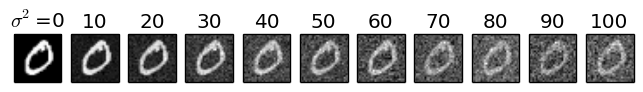
\includegraphics[width=\textwidth]{figs/noisy_row.png}
	\caption{Example of noisy images. As the variance ($\sigma^2$) of the noise distribution increases, the images are considerably more corrupted.}
	\label{fig:noisy}
\end{figure}

\begin{figure}
	\centering
	\begin{minipage}[b]{0.45\textwidth}
		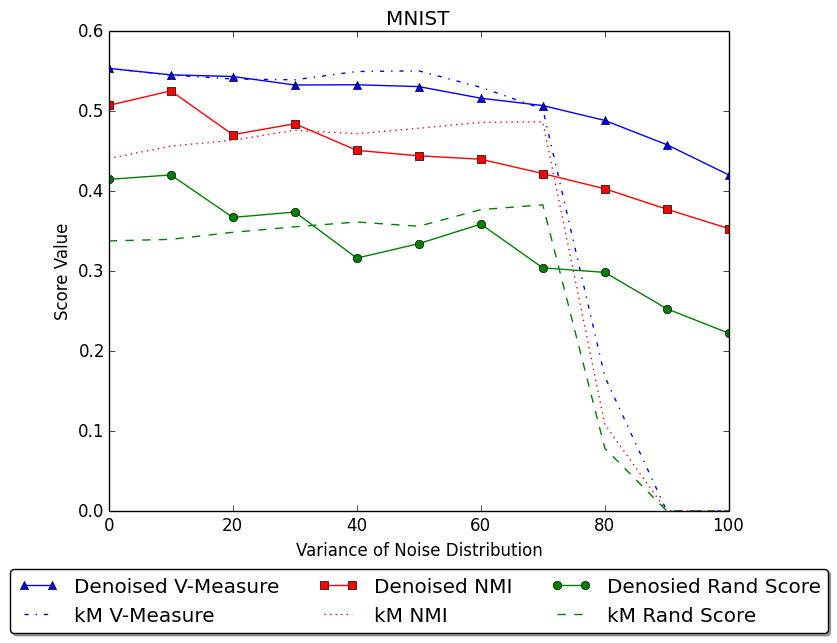
\includegraphics[width=\textwidth]{figs/mnist_noise.png}
	\end{minipage}
	\hfill
	\begin{minipage}[b]{0.45\textwidth}
		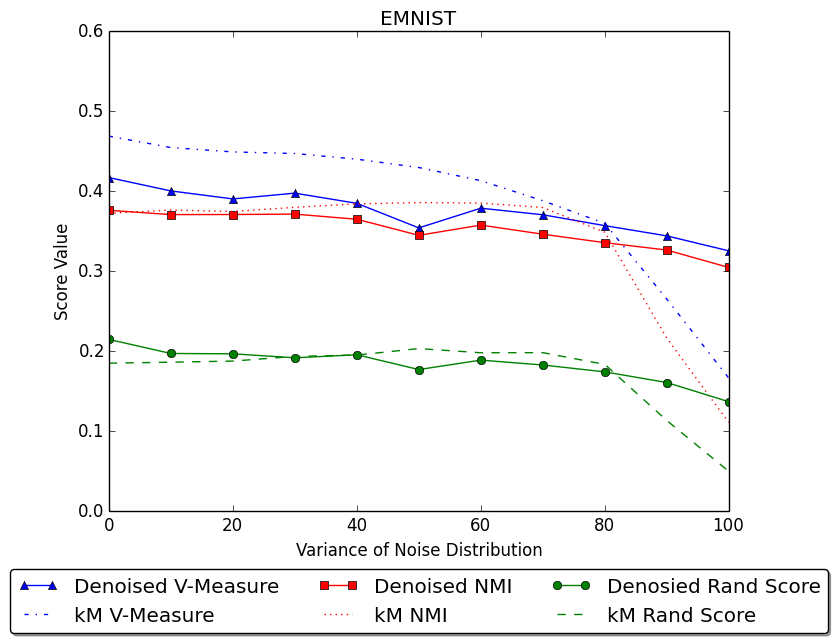
\includegraphics[width=\textwidth]{figs/emnist_noise.png}
	\end{minipage}
	\caption{Effect of noisy data on performance. Solid lines show score values from the clusterings generated by autoencoded $k$-means (with denoising) on noisy data. Dashed lines show score values of clusterings produced by gradient $k$-means (kM) without any autoencoder on the same noisy data.}
	\label{fig:noise}
\end{figure}
